\section{Метод Ньютона-Рафсона}

\textbf{Алгоритм метода}:
$$ x^{k + 1} = x^{k} - t_{k}H^{-1}(x^{k})\nabla f(x^{k}) $$

$d^{k} = -H^{-1}(x^{k})$ --- направление спуска.

$t_{k}$ --- шаг выбирается из условия убывания функции в точках последовательности: $f(x^{k + 1}) < f(x^{k})$.

Основной критерий окончания метода: $||\nabla f(x^{k})|| < \varepsilon$.

Начальные параметры метода: $x^{0}, \varepsilon$.

Изменяемые параметры метода: величина шага $t_{k}$.

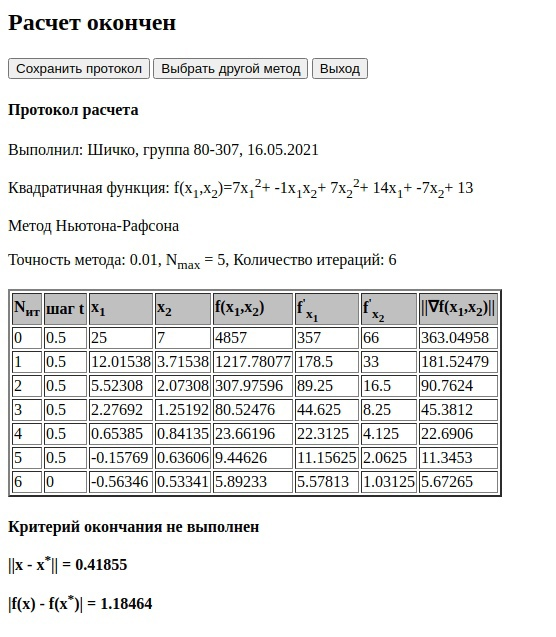
\includegraphics[width=0.8\linewidth]{images/3_prot}\\
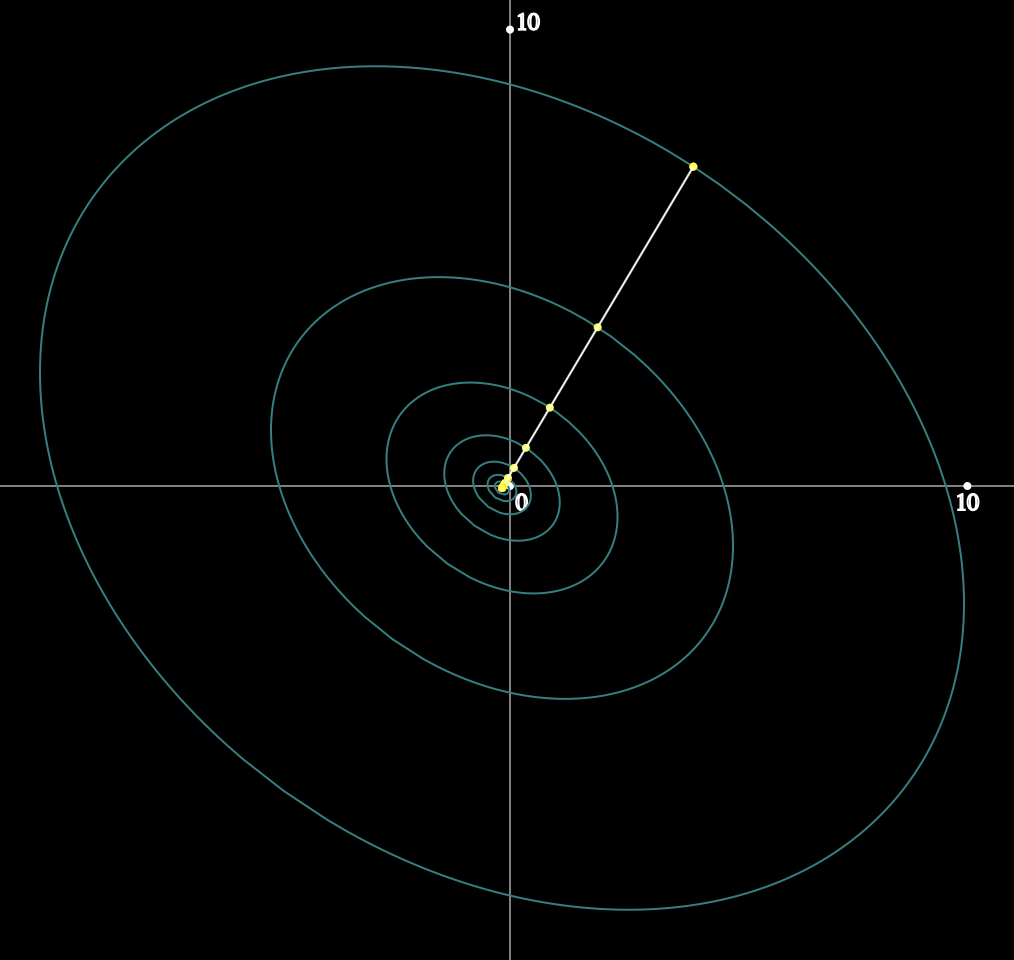
\includegraphics[width=0.8\linewidth]{images/3_graf}\\

\textbf{Последняя итерация}:\\
$x^{14} = x^{13} - t_{13}H^{-1}|x^{13}| \nabla f(x^{13})$\\
$x^{13} = 
\begin{pmatrix}
  -0.18868\\
  -0.03518
\end{pmatrix}
$\\

$t_{13} = 0.5$\\
$ % recalc
H^{-1}(x^{14}) = 
\begin{pmatrix}
  0.078192 & -0.008555\\
  -0.008555 & 0.078192
\end{pmatrix}
$\\

$
\nabla f(x^{13}) = 
\begin{pmatrix}
  10x_{1} + 3x_{2} + 2\\
  12x_{2} + 3x_{1} + 1
\end{pmatrix}
=
\begin{pmatrix}
  0.00769\\
  0.01184
\end{pmatrix}
$\\

$
x^{14} = 
\begin{pmatrix}
  -0.18868\\
  -0.03518
\end{pmatrix}
-
0.5
\begin{pmatrix}
  0.0005\\
  0.00086
\end{pmatrix}
=
\begin{pmatrix}
  -0.18893\\
  -0.03561
\end{pmatrix}
$\\
\pagebreak
